% ============================================================
% 1  Hook: the Kondo effect
% ============================================================
\begin{frame}[t]
\ft{The Kondo effect: a magnetic impurity in a metal}
\begin{columns}[T]
\begin{column}{0.45\textwidth}
\centering
\begin{tikzpicture}[x=0.95cm,y=1.05cm,font=\scriptsize]
 \draw[mygray,rounded corners=4pt] (-2.5,-2.0) rectangle (2.5,2.0);
 % halo (step 2 onward)
 \only<2->{\fill[cKondo,opacity=0.18] (0,0) circle (1.35); \draw[cKondo,dashed] (0,0) circle (1.35);}
 % electrons outside the halo: always the same
 \foreach \x/\y/\d in {-2.1/1.6/1,-1.2/1.65/-1,-0.2/1.7/1,0.9/1.55/-1,1.9/1.6/1,
   -2.15/0.5/-1,2.1/0.7/1,-2.1/-0.6/1,2.15/-0.4/-1,1.9/-1.6/1,
   -1.9/-1.6/-1,-0.9/-1.7/1,0.2/-1.65/-1,1.0/-1.7/1,-1.6/0.9/1,1.55/1.0/-1,-1.6/-1.0/-1,1.65/-0.9/1}{
   \fill[mygraydark] (\x,\y) circle (0.06);
   \draw[->,mygraydark,>=stealth,thick] (\x,\y-0.22*\d) -- (\x,\y+0.22*\d);}
 % electrons inside the halo: mixed in step 1, down from step 2
 \foreach \x/\y/\d in {0.85/0.55/1,-0.8/0.6/-1,-0.95/-0.4/1,0.3/-0.9/-1,0.95/-0.6/1,-0.15/1.0/-1}{
   \fill[mygraydark] (\x,\y) circle (0.06);
   \only<1>{\draw[->,mygraydark,>=stealth,thick] (\x,\y-0.22*\d) -- (\x,\y+0.22*\d);}
   \only<2->{\draw[->,cKondo,>=stealth,thick] (\x,\y+0.22) -- (\x,\y-0.22);}}
 % the impurity
 \draw[cLM,fill=cLM!15,thick] (0,0) circle (0.28);
 \draw[->,cLM,>=stealth,line width=2.2pt] (0,-0.3) -- (0,0.45);
 \only<1>{\node[cLM,font=\small] at (0,-2.4) {local moment};}
 \only<2->{\node[cKondo,font=\small] at (0,-2.4) {Kondo singlet};}
\end{tikzpicture}
\end{column}
\begin{column}{0.53\textwidth}
\vspace{0.2cm}
\onslide<1->{$H = H_{\rm host} + J\,\vec S\cdot\vec s(0)$
\begin{itemize}
 \item Impurity spin coupled to the conduction electrons
\end{itemize}}
\onslide<2->{\begin{itemize}
 \item Low $T$: the electrons rearrange and \colorbox{cKondo!20}{\mystrut screen the moment}
 \item Strong coupling: \colorbox{citron!40}{\mystrut beyond perturbation theory}
\end{itemize}}
\vspace{0.5cm}
\onslide<3->{\centering{\Large $T_K = D\,e^{-1/\tikz[remember picture,baseline=0pt]\coordinate(rho);{\color{cKondo}\rho_0}J}$}\par}
\onslide<3->{\begin{tikzpicture}[remember picture,overlay]
 \node[font=\scriptsize,cKondo,align=center,fill=white] (ann) at ($(rho)+(0.5,-0.8)$) {host density of states\\at the Fermi level};
 \draw[cKondo,->,>=stealth] (ann.north) -- ($(rho)+(0.3,-0.2)$);
\end{tikzpicture}}
\end{column}
\end{columns}
\onslide<3->{\tk{The host density of states decides if, and when, the moment is screened}}
\end{frame}
% Notes: Opening: excellent conference, lots of new physics and numerical methods for moire materials; this talk: magnetic impurities on stacked graphene.
% Notes: Metal: bath electrons rearrange to screen the impurity moment; strong-coupling effect at low T; scale T_K.
% Notes: Punchline of the slide: rho_0 sits in the exponent, so the host DoS decides everything that follows.

% ============================================================
% 2  Graphene
% ============================================================
\begin{frame}[t]
\ft{No Kondo effect in graphene at charge neutrality}\par
\vspace{0.4cm}
\begin{columns}[c]
\begin{column}{0.54\textwidth}
\centering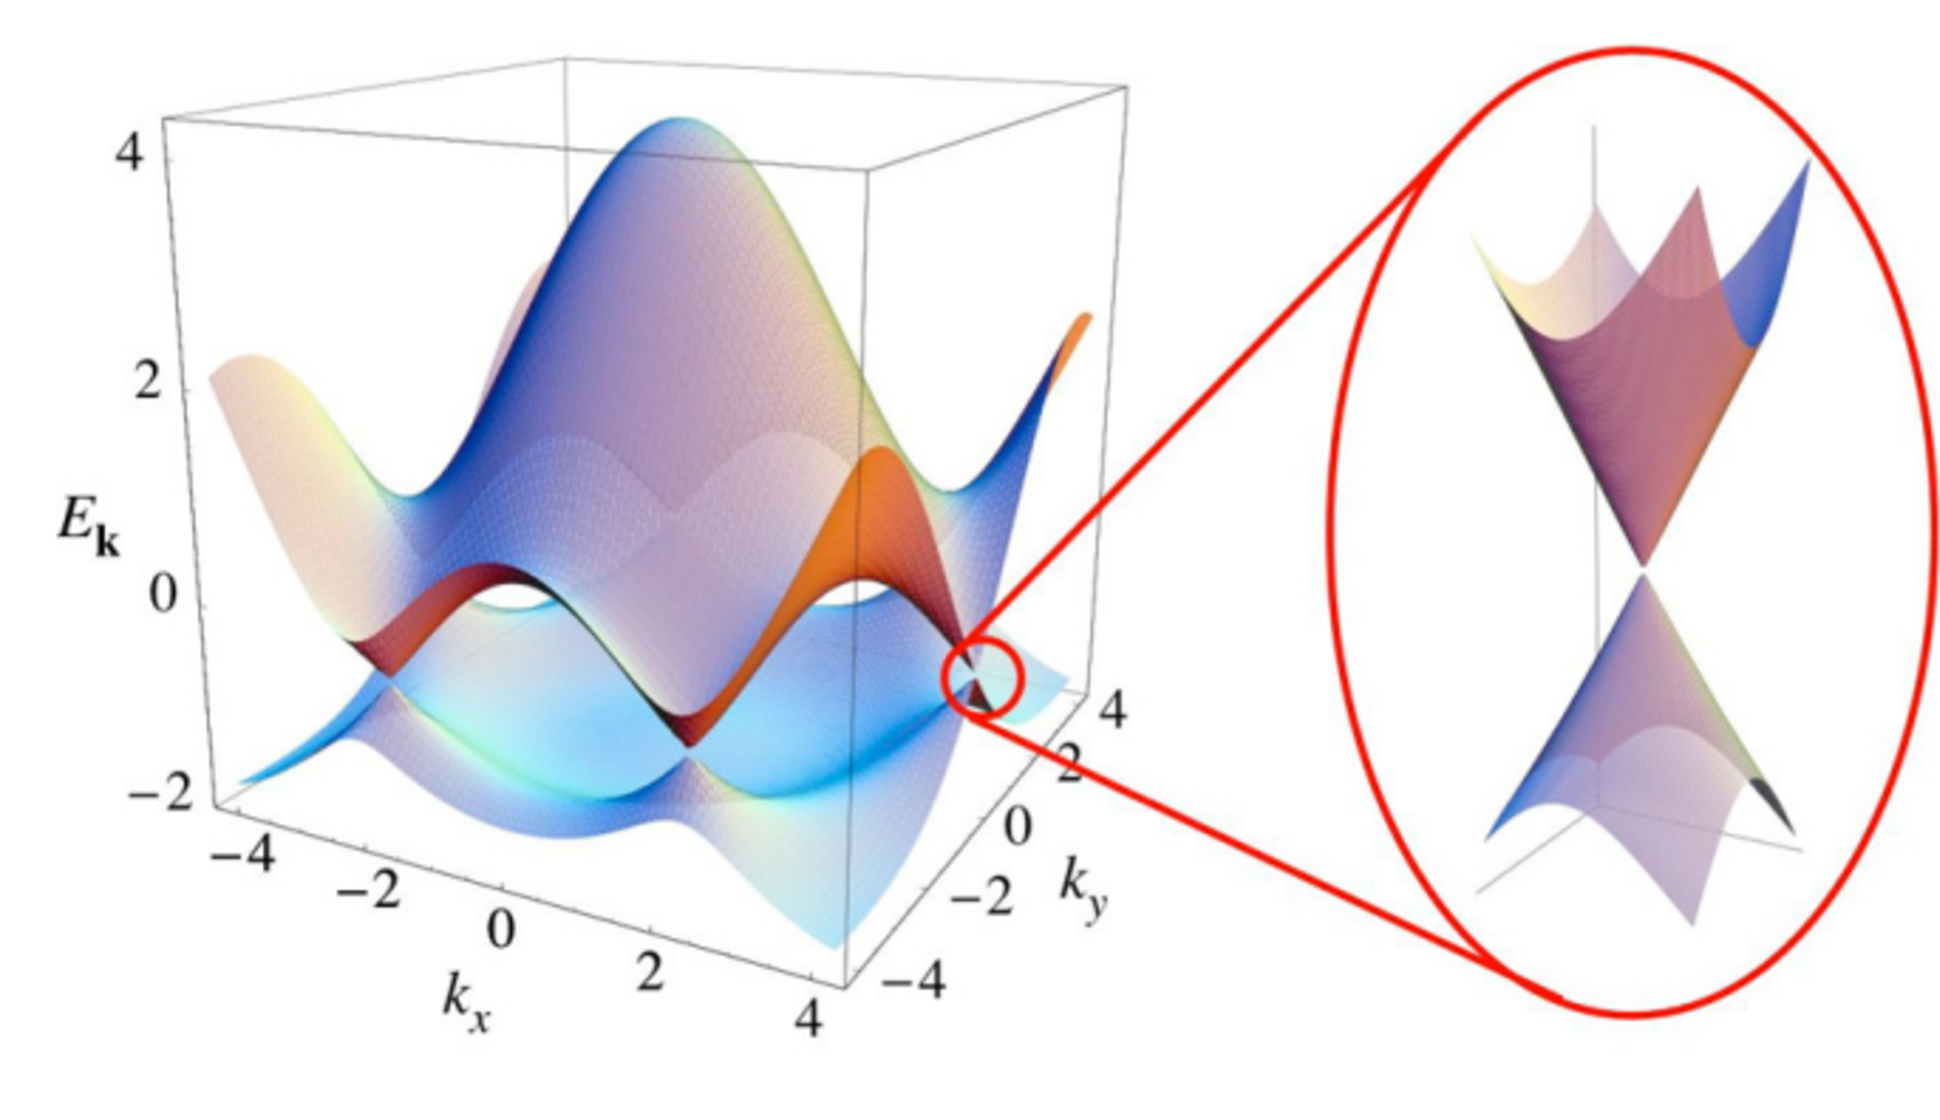
\includegraphics[width=\linewidth]{figures/prev_graphene_cone.png}\\[2pt]
{\tiny\color{citegray} Castro Neto et al., Rev. Mod. Phys. 81, 109 (2009)\par}
\end{column}
\begin{column}{0.44\textwidth}
\centering
\begin{tikzpicture}[font=\small,x=1.0cm,y=1.0cm]
 \fill[spinach!15] (-1.5,0)--(-1.5,1.5)--(0,0)--(1.5,1.5)--(1.5,0)--cycle;
 \draw[->,>=stealth] (-1.8,0)--(1.95,0) node[below]{$\omega$}; \draw[->,>=stealth] (0,0)--(0,1.85) node[left]{$\rho(\omega)$};
 \draw[very thick,spinach] (-1.5,1.5)--(0,0)--(1.5,1.5);
 \fill[cLM] (0,0) circle (0.08);
 \node[cLM,anchor=north] at (0,-0.1) {$\rho(E_F)=0$};
\end{tikzpicture}\\[6pt]
{\Large $T_K = D\,e^{-1/{\color{cLM}\rho_0}J}$}\\[6pt]
{\small ${\color{cLM}\rho_0\to 0}$ \ gives \ $T_K\to 0$\\[3pt] the moment \colorbox{cLM!20}{\mystrut stays free}\par}
\end{column}
\end{columns}
\vspace{0.55cm}
% fixed-size block, appears at step 2
\begin{minipage}[t][1.0cm][t]{\linewidth}\centering
\uncover<2->{\colorbox{tomato!30}{\mystrut Magnetic moments in graphene: experiments}\\[3pt]
{\tiny\color{citegray} H adatoms: González-Herrero et al., Science 352, 437 (2016)\qquad Vacancies: Jiang, \dots, Andrei, Nat. Commun. 9, 2349 (2018)\par}}
\end{minipage}
\tk{What happens in other graphene-like materials?}
\end{frame}
% Notes: Graphene: cone, rho -> 0 at the Fermi level, so no Kondo effect at charge neutrality.
% Notes: Experimentally the moment can be made by adsorbing hydrogen (Brihuega group).
% Notes: Experiments: hydrogen adatoms (Brihuega group) and vacancies (Andrei group) give magnetic moments in graphene.

% ============================================================
% 2b  Model
% ============================================================
\begin{frame}[t]
\ft{Model: Anderson impurity on twisted bilayer graphene}
\par\vspace{0.3cm}
\colorbox{spinach!40}{\mystrut Host} \small Bistritzer--MacDonald continuum model\par
\begin{columns}[c]
\begin{column}{0.60\textwidth}
\scriptsize\setlength\arraycolsep{0.5pt}
\vspace{-12pt}\[ H(\mathbf{k}) = \begin{pmatrix} h^{K}_{\theta/2}(\mathbf{k}) & wT_1 & wT_2 & wT_3 \\ wT_1^\dagger & h^{K}_{-\theta/2}(\mathbf{k}-\mathbf{q}_1) & 0 & 0 \\ wT_2^\dagger & 0 & h^{K}_{-\theta/2}(\mathbf{k}-\mathbf{q}_2) & 0 \\ wT_3^\dagger & 0 & 0 & h^{K}_{-\theta/2}(\mathbf{k}-\mathbf{q}_3) \end{pmatrix} \]
\end{column}
\begin{column}{0.38\textwidth}
\centering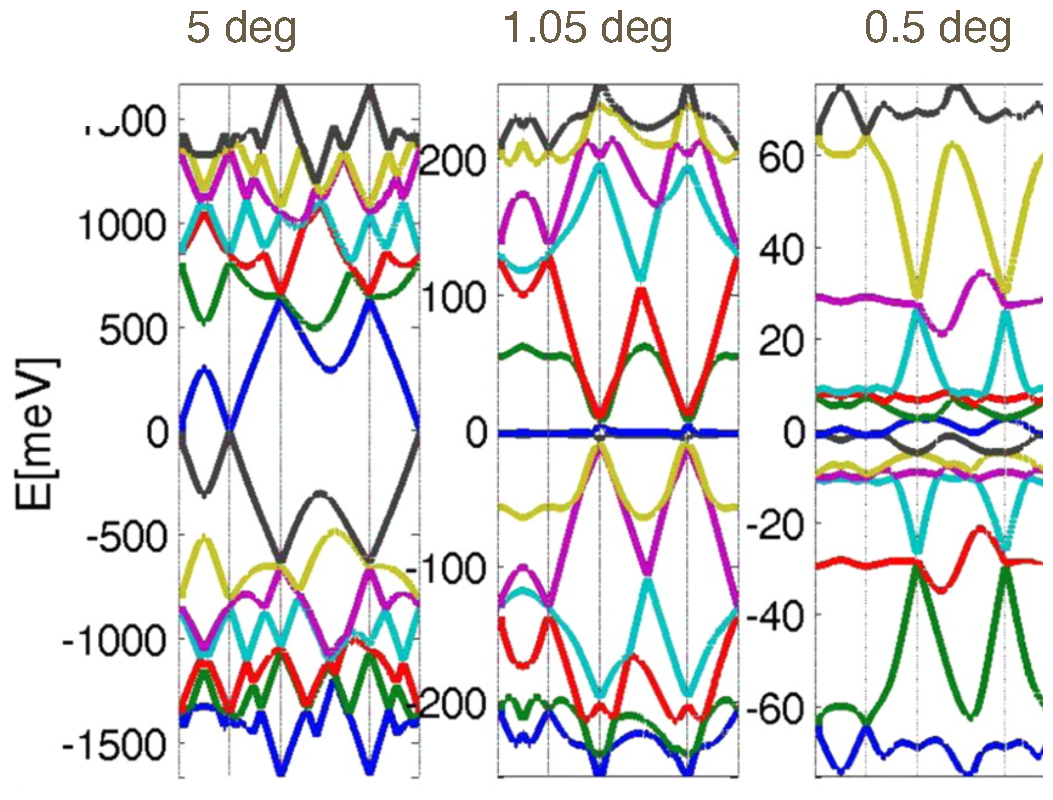
\includegraphics[height=2.8cm]{figures/prev_bm_bands.png}\\[1pt]
{\tiny\color{citegray} Bistritzer and MacDonald, PNAS 108, 12233 (2011)}
\end{column}
\end{columns}
\vspace{0.15cm}
\colorbox{orchid!30}{\mystrut Impurity} \small Anderson model\par
\begin{columns}[c]
\begin{column}{0.37\textwidth}
\centering
% two honeycomb lattices twisted by +-4.5 deg (moire) with a magnetic impurity on top
\begin{tikzpicture}[scale=0.95]
 \clip[rounded corners=6pt] (-2.1,-0.8) rectangle (2.1,0.8);
 \foreach \c/\a in {cKondo!60/4.5,mygraydark!70/-4.5}{\begin{scope}[rotate=\a]
  \foreach \i in {-11,...,11}{\foreach \j in {-11,...,11}{
   \draw[\c,line width=0.2pt] (1.5*0.2*\i,1.732*0.2*\j+0.866*0.2*\i) +(0:0.2) -- +(60:0.2) -- +(120:0.2) -- +(180:0.2) -- +(240:0.2) -- +(300:0.2) -- cycle;
  }}\end{scope}}
 \fill[white] (0,0) circle (0.2); \fill[cLM] (0,0) circle (0.17);
 \draw[white,line width=2.4pt,->,>=stealth] (0,-0.05)--(0,0.65); \draw[cLM,line width=1.2pt,->,>=stealth] (0,-0.05)--(0,0.65);
\end{tikzpicture}
\end{column}
\begin{column}{0.61\textwidth}
\small
\vspace{-10pt}\[ H_{\rm imp} = \epsilon_d \sum_\sigma n_{d\sigma} + U\, n_{d\uparrow} n_{d\downarrow} + V \sum_\sigma \left( d^\dagger_\sigma c^{\phantom\dagger}_{0\sigma} + {\rm h.c.} \right) \]\vspace{-4pt}
\centering
\begin{tikzpicture}[font=\footnotesize,scale=0.9]
 \foreach \x/\t/\c in {0/{|0\rangle}/mygray,1.1/{|\!\uparrow\rangle}/cLM,2.2/{|\!\downarrow\rangle}/cLM,3.3/{|\!\uparrow\downarrow\rangle}/mygray}{
  \node[draw=\c,fill=\c!15,rounded corners=2pt,minimum width=0.9cm,minimum height=0.6cm] at (\x,0) {$\t$};}
\end{tikzpicture}\\[3pt]
\footnotesize 4 states; large $U$ leaves $\uparrow,\downarrow$:\\ a spin-$\tfrac12$ moment, $J\sim V^2/U$
\end{column}
\end{columns}
\vspace{0.1cm}
{\tiny\color{citegray} Impurities in TBG: Shankar, Oriekhov, Mitchell, Fritz, PRB 107, 245102 (2023);\\[-1pt] Chang, Yi, Wu, Kugler, Andrei, Vanderbilt, Kotliar, Pixley, PRL 133, 126503 (2024)}
\end{frame}
% Notes: Quick slide (20 s). Host: BM continuum model, interlayer tunnelling w couples the Dirac cones of the two layers; magic angle 1.05 deg; we stay at charge neutrality.
% Notes: Impurity: Anderson model, particle-hole symmetric (eps_d = -U/2). Four states of the impurity orbital: this is the ln 4 at high temperature on the entropy slide; large U leaves the spin-1/2 moment.

% ============================================================
% 3  Twisted bilayer graphene
% ============================================================
\begin{frame}[t]
\ft{van Hove singularities in the flat band}
\par\vspace{0.45cm}
\begin{columns}[c]
\begin{column}{0.61\textwidth}
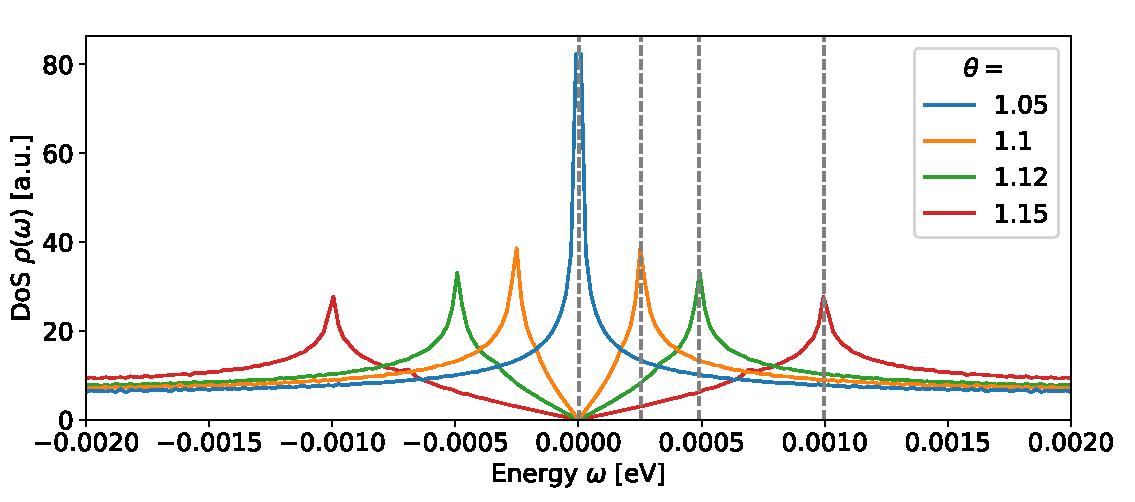
\includegraphics[width=\linewidth]{figures/tbg_fig1b.png}
\end{column}
\begin{column}{0.37\textwidth}
\raggedright
\onslide<1->{Dirac cone at $\omega=0$: $\rho\sim|\omega|$\par\medskip}
\uncover<2->{\colorbox{citron!60}{\mystrut van Hove peaks} at $\pm E_v$\par\medskip}
\uncover<3->{$1.05^\circ$: \colorbox{pumpkin!60}{\mystrut the peaks merge}}
\end{column}
\end{columns}
\vspace{0.1cm}
% fixed-size box, content swaps
\begin{minipage}[t][3.5cm][t]{\linewidth}\centering
\only<2>{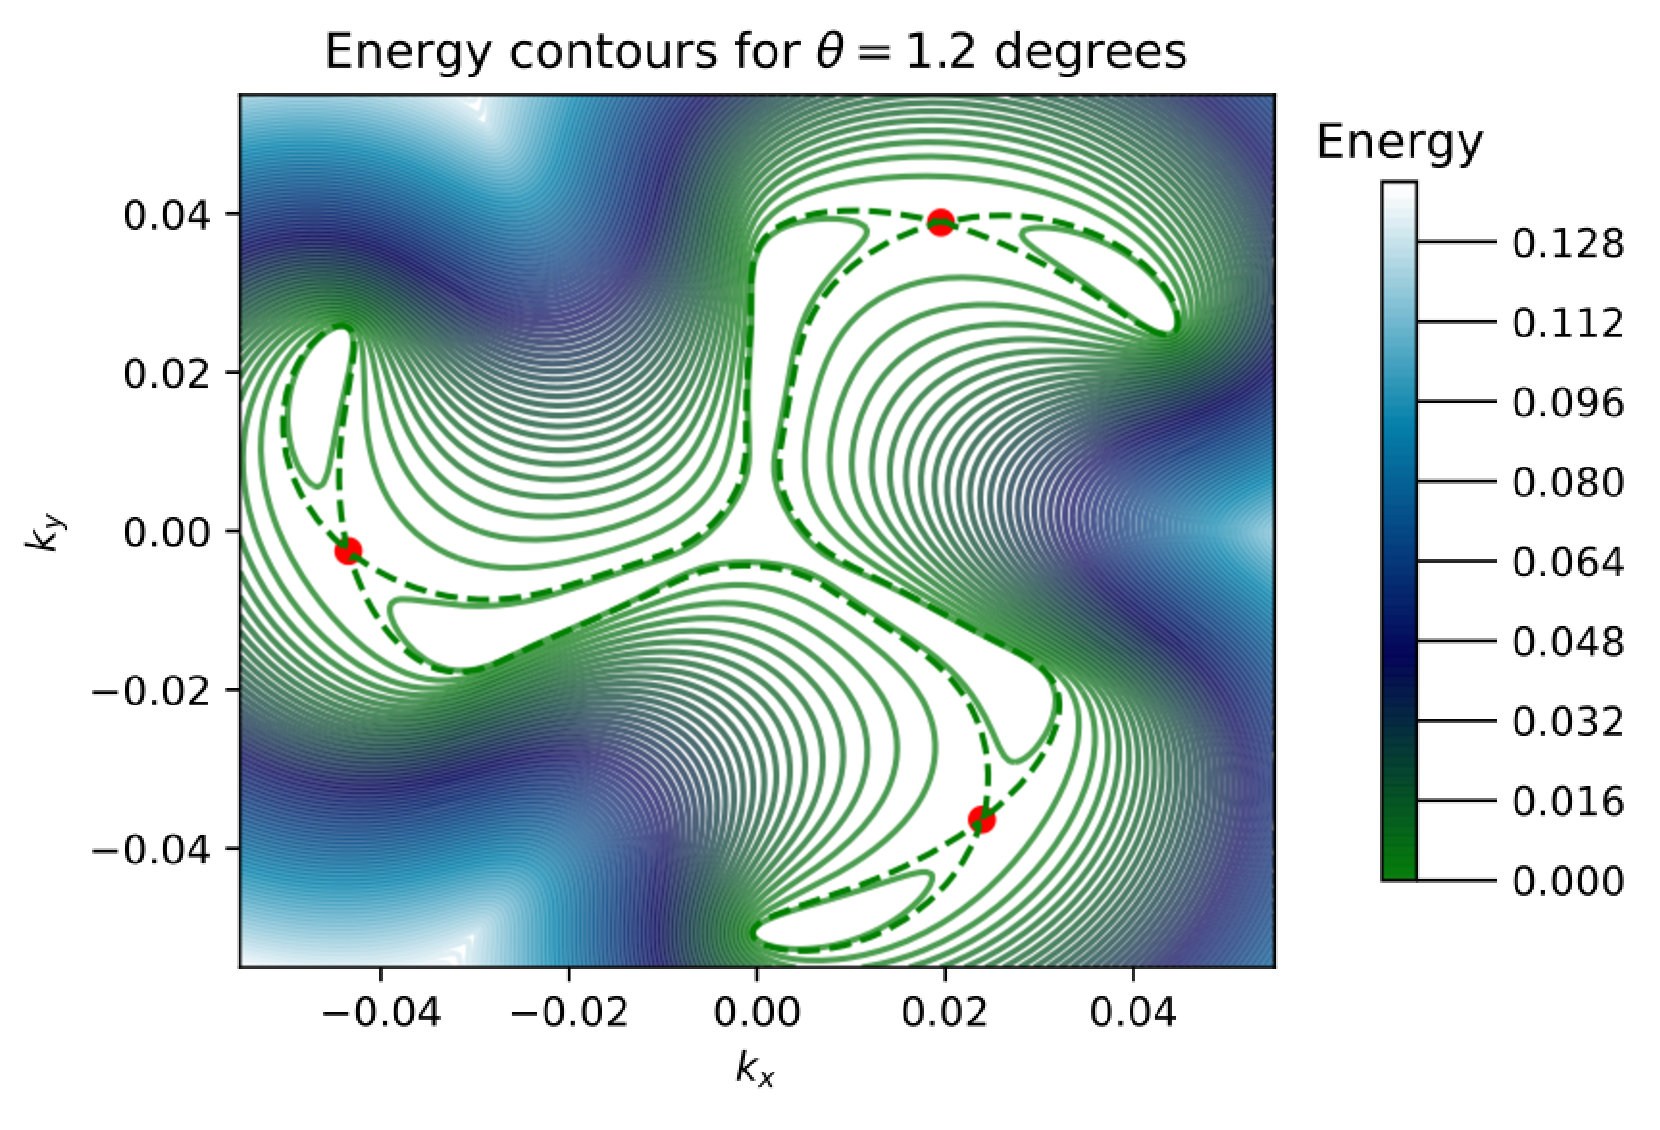
\includegraphics[height=2.7cm]{figures/prev_contours_tbg.png}\hspace{0.3cm}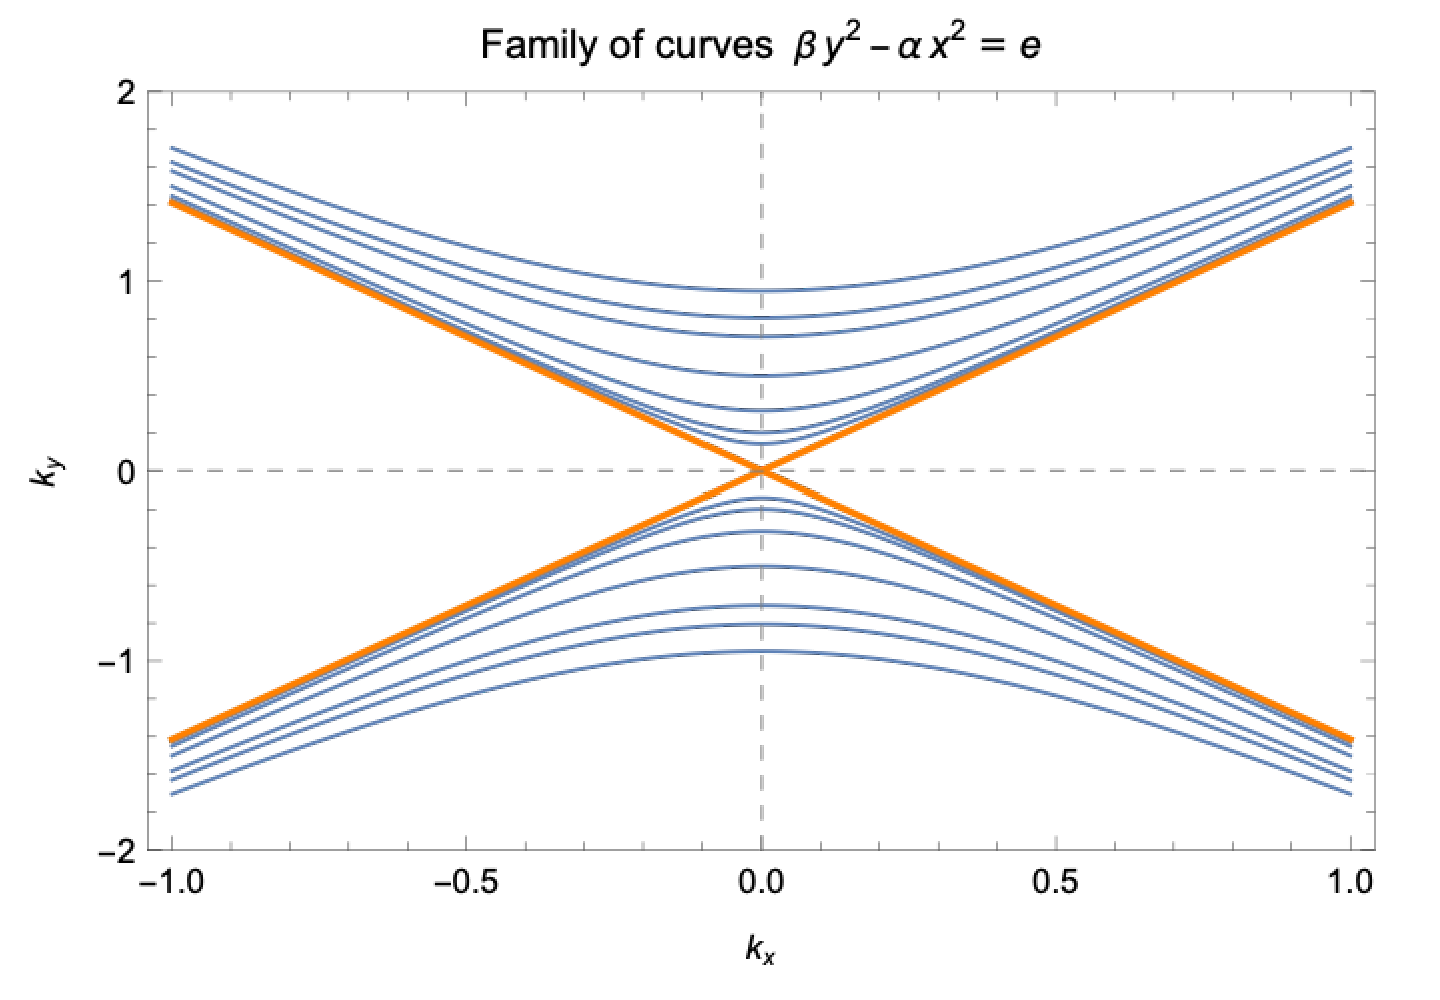
\includegraphics[height=2.7cm]{figures/prev_saddle_log.png}\\[4pt]
\small\colorbox{citron!60}{\mystrut ordinary saddle} \quad $E = E_v + \alpha p_x^2 - \beta p_y^2 \ \Longrightarrow\ \rho(E)\sim\log\left|\frac{\Lambda}{E-E_v}\right|$}
\only<3>{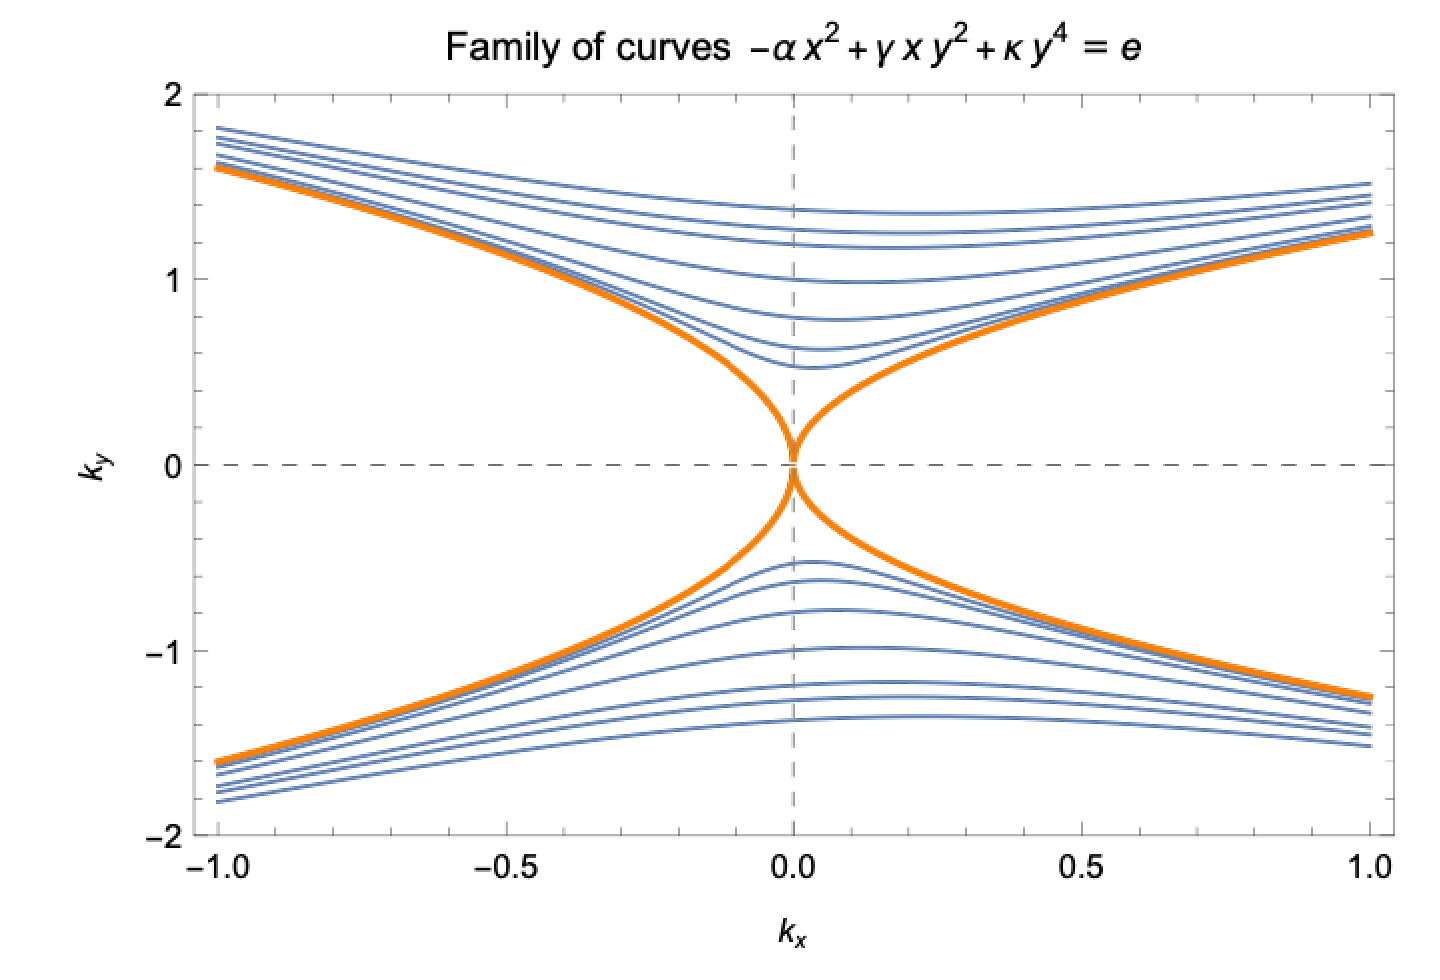
\includegraphics[height=2.7cm]{figures/prev_saddle_higher.png}\hspace{0.3cm}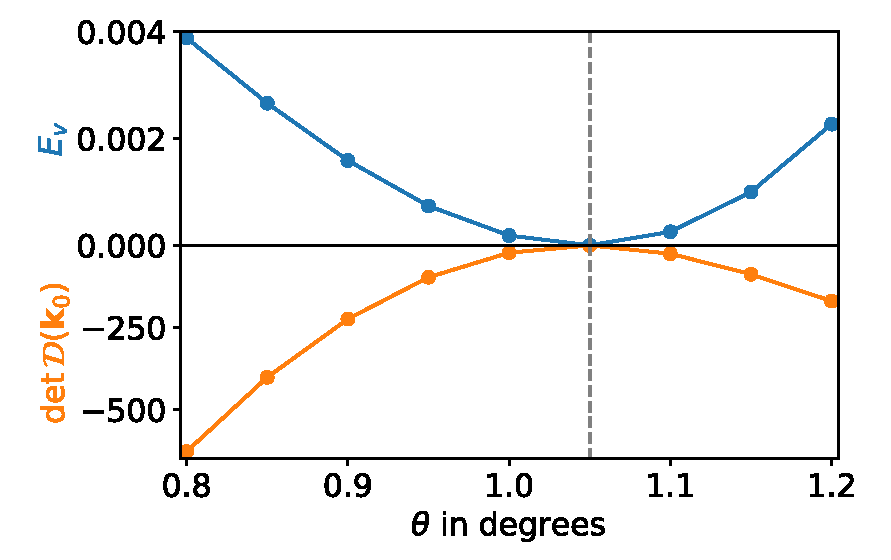
\includegraphics[height=2.7cm]{figures/tbg_fig1c.png}\\[4pt]
\small\colorbox{pumpkin!60}{\mystrut higher-order saddle} \quad $E = \alpha p_x^2 + \gamma p_x p_y^2 + \kappa p_y^4 \ \Longrightarrow\ \rho(E)\sim|E|^{-1/4}$\\[1pt]
{\tiny\color{citegray} Yuan, Isobe, Fu, Nat. Commun. 10, 5769 (2019)}}
\end{minipage}
\onslide<3->{\tk{At $1.05^\circ$ the two vHs merge into a higher-order vHs}}
\end{frame}
% Notes: Bistritzer-MacDonald continuum model; impurity on the surface.
% Notes: Away from the magic angle: Dirac pseudogap at low energy, two log vHs at +-E_v from ordinary saddle points.
% Notes: At 1.05 deg the saddles merge: higher-order vHs, power-law divergence |omega|^(-1/4).

% ============================================================
% 4  vHs boosts T_K
% ============================================================
\begin{frame}[t]
\ft{A van Hove peak boosts $T_K$}
\par\vspace{0.5cm}
\centering
\small
\setlength{\tabcolsep}{3pt}
\renewcommand{\arraystretch}{1.4}
\begin{minipage}[t][3.8cm][t]{\linewidth}\centering
\only<1>{\begin{tabular}{>{\raggedright}p{1.9cm} >{\raggedright}p{3.5cm} >{\centering}p{2.5cm} >{\centering\arraybackslash}p{2.0cm}}
\hline
 & \multicolumn{1}{c}{Density of states $\rho(\omega)$} & $T_K$ & $S_{\rm imp}(T\to 0)$ \\
\hline
Metal & $\rho_0$ : constant & $D\,e^{-1/\rho_0 J}$ & $0$ \\
\rowcolor{cLM!12} Dirac cone & $\rho_0|\omega|$ : linear pseudogap & $T_K = 0$ & $\ln 2$ \\
Standard\newline van Hove & $\rho_0\,[1 + a\ln(D/|\omega|)]$ :\newline log divergence & $D\,e^{\frac1a-\frac1a\sqrt{1+\frac{2a}{\rho_0 J}}}$ & $0$ \\
Higher-order\newline van Hove & $\rho_0|\omega|^{-\alpha}$ :\newline power-law divergence & $D\left(1+\frac{\alpha D^{\alpha}}{\rho_0 J}\right)^{-1/\alpha}$ & $-2\alpha\ln 2$ \\
\hline
\end{tabular}}
\only<2>{\begin{tabular}{>{\raggedright}p{1.9cm} >{\raggedright}p{3.5cm} >{\centering}p{2.5cm} >{\centering\arraybackslash}p{2.0cm}}
\hline
 & \multicolumn{1}{c}{Density of states $\rho(\omega)$} & $T_K$ & $S_{\rm imp}(T\to 0)$ \\
\hline
Metal & $\rho_0$ : constant & $D\,e^{-1/\rho_0 J}$ & $0$ \\
\rowcolor{cLM!12} Dirac cone & $\rho_0|\omega|$ : linear pseudogap & $T_K = 0$ & $\ln 2$ \\
\rowcolor{cKondo!12} Standard\newline van Hove & $\rho_0\,[1 + a\ln(D/|\omega|)]$ :\newline log divergence & $D\,e^{\frac1a-\frac1a\sqrt{1+\frac{2a}{\rho_0 J}}}$ & $0$ \\
\rowcolor{cKondo!12} Higher-order\newline van Hove & $\rho_0|\omega|^{-\alpha}$ :\newline power-law divergence & $D\left(1+\frac{\alpha D^{\alpha}}{\rho_0 J}\right)^{-1/\alpha}$ & $-2\alpha\ln 2$ \\
\hline
\end{tabular}}
\end{minipage}\\[2pt]
{\tiny\color{citegray} Mitchell, Vojta, Bulla, Fritz, PRB 88, 195119 (2013)}
\vspace{0.55cm}
\begin{itemize}\normalsize\raggedright
 \uncover<2->{\item Logarithmic vHs: $T_K$ \colorbox{cKondo!12}{\mystrut enhanced} over the metal}
 \uncover<2->{\item Higher-order vHs: $T_K$ grows as a \colorbox{cKondo!12}{\mystrut power law} in $J$}
\end{itemize}
\onslide<2->{\tk{In TBG the cone and the vHs sit within a few meV of each other: which one wins?}}
\end{frame}
% Notes: Table built from what we already said: metal row = slide 1, Dirac row = slide 2; new rows are the van Hove ones.
% Notes: Last column (entropy) is explained on the next slide.
% Notes: Competition of two singular features on nearby scales: needs a non-perturbative method.

% ============================================================
% 5  NRG and the impurity entropy
% ============================================================
\begin{frame}[t]
\ft{NRG: read the answer off the impurity entropy}
\centering
\raisebox{-0.2cm}{\begin{tikzpicture}[font=\scriptsize,x=0.85cm,y=0.85cm]
 \begin{scope}
  \draw[->] (0,0)--(2.6,0) node[right]{$\omega$}; \draw[->] (1.3,0)--(1.3,1.5) node[right]{$\rho(\omega)$};
  \draw[very thick,spinach] plot[domain=-1.2:1.2,samples=40] ({1.3+\x},{0.15+0.35*abs(\x)+0.45/(1+30*\x*\x)});
  \node at (1.3,-0.5) {\textbf{1.} host DoS $\rho(\omega)$};
 \end{scope}
 \draw[-{Stealth},thick] (3.4,0.7)--(4.0,0.7);
 \begin{scope}[xshift=4.3cm]
  \node[circle,draw=cLM,fill=cLM!25,inner sep=2pt] (imp) at (0,0.7) {$S$};
  \foreach \k/\r in {1/0.17,2/0.15,3/0.12,4/0.09,5/0.07}{
    \node[circle,draw=cKondo,fill=cKondo!25,inner sep=0pt,minimum size={2*\r cm}] (c\k) at ({0.45+0.4*\k},0.7) {};}
  \draw (imp)--(c1)--(c2)--(c3)--(c4)--(c5);
  \node at (1.5,0.2) {$t_n\sim\Lambda^{-n/2}$};
  \node at (1.2,-0.5) {\textbf{2.} Wilson chain, solved iteratively};
 \end{scope}
 \draw[-{Stealth},thick] (8.2,0.7)--(8.8,0.7);
 \node[anchor=west] at (8.9,0.7) {\textbf{3.} $S_{\rm imp}(T)$};
\end{tikzpicture}}
\begin{columns}[T]
\begin{column}{0.6\textwidth}
\centering
\begin{tikzpicture}[font=\footnotesize,x=0.61cm,y=2.2cm]
 \draw[->] (0,0)--(9.3,0) node[right]{$\ln T$}; \draw[->] (0,0)--(0,1.65) node[above]{$S_{\rm imp}$};
 \draw[dashed,mygray] (0,1.386)--(9.0,1.386) (0,0.693)--(9.0,0.693);
 \node[left] at (0,1.386) {$\ln 4$}; \node[left] at (0,0.693) {$\ln 2$}; \node[left] at (0,0) {$0$};
 \draw[very thick,mygraydark] (0.1,0)--(2.9,0) .. controls (3.9,0) and (3.7,0.693) .. (4.7,0.693)--(5.9,0.693) .. controls (6.9,0.693) and (6.7,1.386) .. (7.7,1.386)--(9.0,1.386);
 \onslide<2->{\node[anchor=south east] at (9.0,1.42) {$N=4$: empty, $\uparrow$, $\downarrow$, $\uparrow\downarrow$};}
 \onslide<3->{\node[anchor=south east,cLM,align=right] at (5.8,0.73) {$N=2$: $\uparrow$, $\downarrow$\\free moment};}
 \onslide<4->{\node[anchor=south west,cKondo,align=left] at (0.1,0.05) {$N=1$:\\Kondo singlet};
   \draw[dotted,thick,cKondo] (3.8,0)--(3.8,0.693); \node[cKondo,below] at (3.8,0) {$T_K$};}
\end{tikzpicture}
\end{column}
\begin{column}{0.38\textwidth}
\vspace{0.3cm}
\begin{itemize}\small\raggedright
 \onslide<1->{\item A plateau at \colorbox{citron!40}{\mystrut $\ln N$: $N$ states} available to the impurity}
 \uncover<4->{\item A step between plateaus: a \colorbox{cKondo!20}{\mystrut screening scale}, here $T_K$}
 \uncover<4->{\item \colorbox{citron!40}{\mystrut $S_{\rm imp} = S_{\rm total} - S_{\rm host}$}}
\end{itemize}
\end{column}
\end{columns}
\onslide<4->{\tk{This curve is the one diagnostic used for the rest of the talk}}
\end{frame}
% Notes: Input to NRG is only the host DoS. Log-discretise, map to a Wilson chain with hopping decaying as Lambda^(-n/2), diagonalise iteratively: numerically exact, non-perturbative.
% Notes: Read from high T to low T: ln4 = four states of the impurity orbital, ln2 = free spin, 0 = singlet.
% Notes: Never use the letter S for the number of states; it is N.
% Notes: Negative values are allowed because the host contribution is subtracted (needed for the next slide).

% ============================================================
% 6  The result
% ============================================================
\begin{frame}[t]
\ft{Kondo revival at the magic angle}
\par\vspace{0.45cm}
\centering
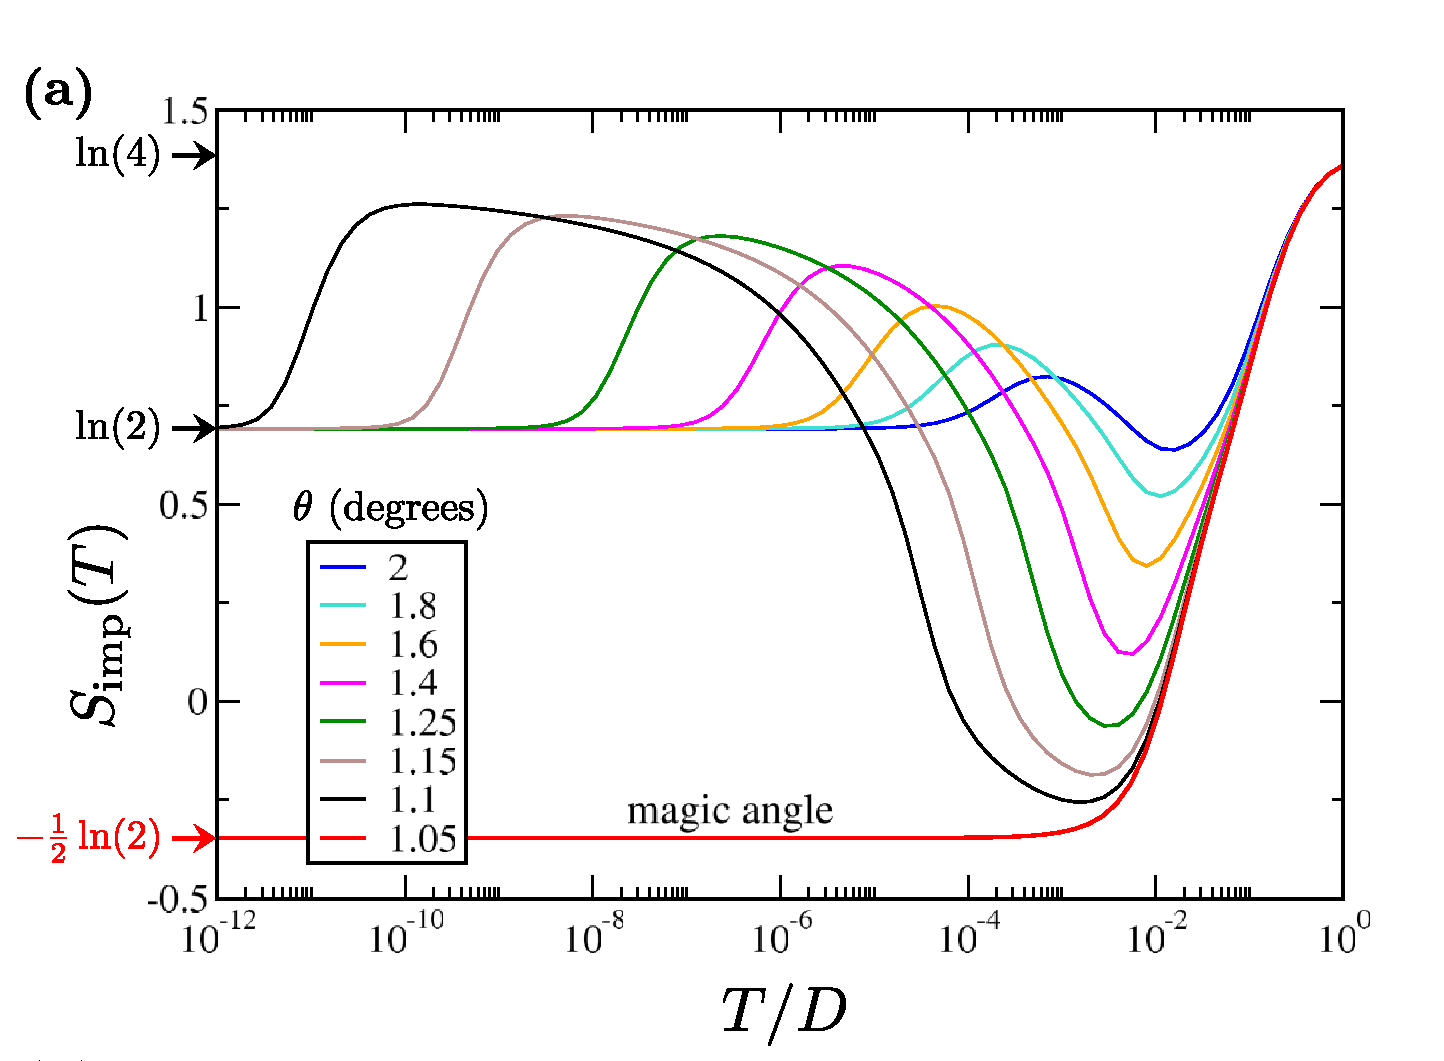
\includegraphics[height=4.3cm]{figures/tbg_fig4a.png}\hfill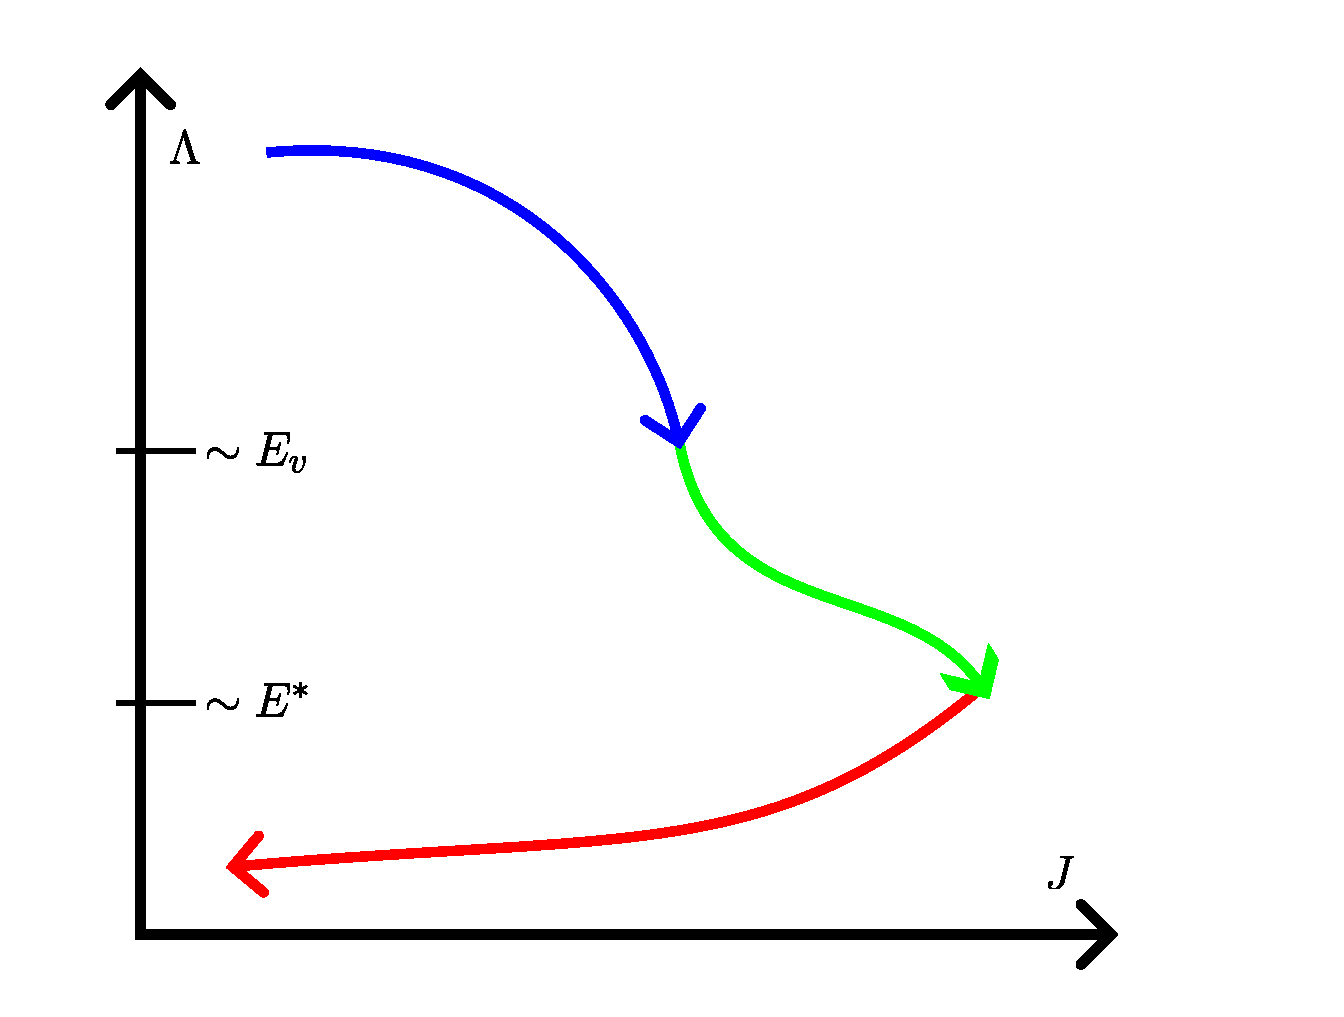
\includegraphics[height=4.3cm]{figures/tbg_fig5.png}\par
\vspace{2pt}
{\tiny\color{citegray} Shankar, Oriekhov, Mitchell, Fritz, PRB 107, 245102 (2023)}\\[-2pt]
{\tiny\color{citegray} See also: Chang, Yi, Wu, Kugler, Andrei, Vanderbilt, Kotliar, Pixley, PRL 133, 126503 (2024)}\par
\vspace{4pt}
\small\onslide<1->{Screening begins at $E_v$; below $E^*\sim|E_v|^3$ the cone wins: \colorbox{cLM!20}{\mystrut moment unscreened}\par}
\vspace{2pt}
\uncover<2->{Magic angle: $E_v,\,E^*\to 0$, the cone never wins: \colorbox{cKondo!20}{\mystrut moment screened}}
\onslide<2->{\tk{One impurity is only the dilute limit. What happens when two sit close together?}}
\end{frame}
% Notes: Away from the magic angle: flow HO-vHs -> log vHs -> Dirac; entropy dips, overshoots to ln4, ends at ln2: free moment below E*.
% Notes: Exactly at 1.05 deg the cone is squeezed out and the impurity is screened: revival of the Kondo effect, S = -1/2 ln2.
% Notes: Bridge to Bernal bilayer: you never have just one impurity; Kondo is the dilute limit; two nearby impurities bring in RKKY, which competes with Kondo.
